\documentclass[12pt, a4paper]{article}
\usepackage{amssymb}
\usepackage{amsmath}
\usepackage{amsthm}
\usepackage{graphicx}
% \usepackage{authblk}
\usepackage{float}
\usepackage{subfig}
\usepackage{epsfig}
% \usepackage{subfigure}
\usepackage{setspace}
\usepackage{geometry}
\geometry{left=2cm,right=2cm,top=2cm,bottom=2cm}

\usepackage{tabularx}

\usepackage[usenames,dvipsnames]{xcolor}
\usepackage[colorlinks=true,linkcolor=black,citecolor=BlueViolet,urlcolor=Maroon]{hyperref}
% \usepackage{caption}
% \usepackage{subcaption}
% \usepackage{enumerate}
\usepackage{tikz}
 
\title{COMP6706 Report: Towards More Accurate Fingerprint Recognition Using Deep Learning and Graph Matching}
\author{
    Cao Pei (20031287R) \\
    \text{peipei.cao@connect.polyu.hk}
    \and 
    Feng Yulin (18070059R) \\
    \text{yulin.feng@connect.polyu.hk}
}

\date{}

\newcommand{\horrule}[1]{\rule{\linewidth}{#1}}
\newcommand{\entit}{COMP6706 Report: Towards More Accurate Fingerprint Recognition Using Deep Learning and Graph Matching}
\newcommand{\numword}{Number of Words: }

\begin{document}
\begin{titlepage}
    \begin{center}
        \horrule{0.5pt} \\ [0.4cm]
        \vspace{-1.5ex}
        { \bfseries \entit \\ \vspace{0.4cm}}
          \horrule{2pt} \vspace{-2ex}
        \numword \\
    \end{center}

    \vspace{3cm}
    \begin{table}[h]
        \centering
        \begin{tabular}{p{3cm}<{\raggedleft} p{6cm}<{\centering}}
          Name:  & {Cao Pei}            \\
          Student ID:  & {20031287R}          \\
          Email:  & {peipei.cao@connect.polyu.hk} \\
        \end{tabular}
    \end{table}

    \vspace{3cm}
    \begin{table}[h]
        \centering
        \begin{tabular}{p{3cm}<{\raggedleft} p{6cm}<{\centering}}
          Name:  & {Feng Yulin}            \\
          Student ID:  & {18070059R}          \\
          Email:  & {yulin.feng@connect.polyu.hk} \\
        \end{tabular}
    \end{table}

\end{titlepage}

\newpage

\begin{spacing}{1} 
    % \maketitle   

    \begin{abstract}
    This paper
\end{abstract}
    \section{Introduction}
Fingerprint used for human identification can be dated back to over one hundred years ago when people found that no two individuals shared the same fingerprints. Fingerprint was used in forensics since criminals usually unintentionally left their fingerprints in crime scenes and their fingerprints can be used as evidence against themselves. These applications calls for the use of fingerprint and thus research on fingerprint recognition. Compared with other biometrics such as face, iris and voice, fingerprint is highly distinctive, permanent, easy to accept and easy to collect \cite{Maltoni2009}. This makes fingerprint one of the most popular biometrics which is used in a large number of recognition domains such as healthcare, electronic payment, border crossing and forensics.

Because manual fingerprint recognition requires human experts to match fingerprint one by one, the cost of training such experts is high, and matching fingerprint with fingerprints in the database is time consuming and slow, the demand for automatic fingerprint recognition is growing quickly. This makes fingerprint recognition a popular pattern recognition research problem which has attracted significant attention from both the academia and industry. Although many fingerprint recognition solutions have been proposed and showed their effectiveness over the past few decades, fingerprint recognition is still challenging especially for low quality fingerprints due to fingerprint noise and distortion. Therefore, it is an intriguing  research problem even till nowadays, and accurate and fast fingerprint recognition algorithm is in demand.

Generally speaking, the fingerprint images can be classified as 3 categories: plain, latent and rolled \cite{nimkarFingerprintSegmentationAlgorithms2014}.
The plain fingerprint images are usually acquired by touching the fingers on a flat surface.
The latent images are usually collected from some real crime scenes, therefore is usually low quality and contains a lot of noise.
And the rolled fingerprint images are often collected by rolling the fingers from one side to another, which can keep most of the fingerprint ridge information \cite{nimkarFingerprintSegmentationAlgorithms2014}.

There are seven kinds of main factors which is responsible for the intra-class variations: displacement, rotation, partial overlap, non-linear distortion, press and skin condition,  noise and feature extraction errors \cite{Maltoni2009}.
The most important and difficult factor is the non-linear distortion problem. This kind of error is generated on the process of sensing  the 3D fingerprint shapes into a 2D flat surface. Most fingerprint matching algorithms usually do not consider such variations, and consider the obtained fingerprint images as non-distorted by assuming that it was produced by a correct finger placement. Fingerprint recognition can be divided into two parts: fingerprint segmentation and fingerprint matching. Fingerprint segmentation is the process which extract the foreground regions from the original fingerprint images \cite{Maltoni2009}. There are many different kinds of segmentation methods and in this survey and project, we will use segmented images and will only concentrate on the matching part. In the following survey details  part, we will introduce some newly published deep learning-based fingerprint recognition algorithms.

Fingerprint recognition, also called fingerprint matching, can basically be divided into two categories: minutiae based matching and non-minutiae based matching. Minutiae is considered as stable and robust local fingerprint ridge characteristics. Minutiae is usually represented by location, orientation, and minutiae type (i.e., ridge endings and ridge bifurcations). Therefore, minutiae based matching methods try to align two fingerprints by matching the largest number of corresponding minutiae pairs. For low quality fingerprint when it is difficult to extract minutiae, non-minutiae based matching comes into play. Some other fingerprint features such as ridge orientation, ridge frequency,  and ridge shape. To date, most fingerprint recognition algorithms are based on minutiae because of its stability and robustness.

Conventional minutiae based fingerprint recognition method considers matching minutiae pairs by comparing minutiae between two fingerprints. The fast development and increasing popularity of deep learning methods shows remarkable progress in computer vision tasks. Some challenging biometric problems, such as face recognition \cite{SchroffCVPR2015facenet} and iris recognition \cite{ZhaoICCV2017}, have achieved great success thanks to deep learning based methods. There are also some works on using deep learning based methods for fingerprint matching and research shows that deep learning method can also improve fingerprint matching in some scenarios. As another popular research area, graph neural network has also made significant progress over the last decade. Since minutiae of one fingerprint can be formulated as a graph, this implies the possibility of applying graph neural network for matching minutiae graphs. 

This paper is organized as follows: we first discuss and compare related work in Section \ref{sec:related}. Section \ref{sec:method} presents our methods for fingerprint recognition and the corresponding experiment result is shown in Section \ref{sec:experiment}. Conclusion and future work is in Section \ref{sec:conclusion}.
    \section{Related Work}
\label{sec:related}

\subsection{Conventional Fingerprint Recognition Method}
Minutiae based method is the most widely used method for fingerprint recognition. Consider two fingerprint images with M and N minutiae respectively. Each minutiae is represented by location, orientation and type. A solution is required to match as many minutiae pairs as possible. To achieve this goal, local minutiae structures are formed to match minutiae. Compared with global minutiae matching \cite{ChikkerurICB2006}, local minutiae matching are computationally cheaper and more robust against fingerprint distortion. Earlier approaches can be found in \cite{HrechakPR1990} and \cite{KovacsTPAMI2000}. To describe local minutiae structure, two methods were proposed: nearest neighbor based and fixed radius based. For nearest neighbor based method, the number of neighbors is fixed \cite{JiangICPR2000} so each minutiae has same number of nearest neighbors. For fixed radius method, a radius is given so that all minutiae that fall within the circle defined by the minutiae as the center and the radius are included \cite{CappelliTPAMI2010mcc}. However, both approaches have their own drawbacks. Nearest neighbor method suffers from missing minutiae and spurious minutiae. Although fixed length method alleviates the issue of missing minutiae and spurious minutiae, it has potential border issues, which means that the minutiae near the border of the circle should be properly treated.

\subsection{Deep Learning Method for Fingerprint Recognition}
The past decade has witnessed the great progress of deep learning in computer vision and pattern recognition \cite{HeCVPR2016ResNet} \cite{Simonyan2014VGG} \cite{SzegedyCVPR2015InceptionV1}. The name “deep learning” is derived from the architecture of deep artificial neural networks, which belongs to the family of machine learning methods. Compared with traditional neural networks which have only one or two layers, deep neural network can have tens or hundreds of layers. Such great progress of deep learning has also facilitated not only the research on fingerprint matching \cite{CaoTPAMI2018}, but also the research on other fingerprint recognition related tasks, such as minutia extraction \cite{TangIJCB2017} \cite{NguyenICB2018}. \cite{LinTIFS2018} did the pioneering work on matching with contactless and contact-based 2D fingerprint with convolutional neural network (CNN), while \cite{LinPR2018} also used CNN to match 3D fingerprint, and both works showed that fingerprint recognition with CNN based method can achieve outperforming results. Instead of extracting minutiae for fingerprint matching, \cite{EngelsmaTPAMI2019} trained a deep neural network to extract fixed-length fingerprint descriptor and regarded minutiae extraction as one step to achieve the final fixed-length representation.

\subsection{Graph Neural Network}
Minutiae of one fingerprint can be formulated as a graph by connecting each minutiae based on some predefined rules. However, due to fingerprint noise and distortion, minutiae graph matching can achieve as good performance as other minutiae based matching method \cite{ChikkerurICB2006}. There is another related research area called graph neural network (GNN).The success of deep neural networks has also boosted the research on graph neural network  in recent years \cite{WuTNNLS2020} \cite{ZhouAI2020} \cite{XuICLR2019GIN}. Compared with images that are structured data, there are also unstructured data in the real world, such as social networks, molecules, and citation networks. Deep neural networks have some limitations to model such kind of data, but graph neural networks show their own flexibility. Motivated by CNN, there is a similar graph convolutional networks called GCN \cite{KipfICLR2017}. A graph is represented by nodes and edges. For classification task, it can be divided in to node level based classification and graph level based classification. GNN can also be used for graph matching \cite{ZanfirCVPR2018} \cite{LiICML2019}. Graph matching is an NP-hard problem, and thus requires complex matching algorithm. \cite{SarlinCVPR2020superglue} formulated graph matching as optimal transport problem which can be solved an efficient approximation algorithm called Sinkhorn algorithm \cite{CuturiNIPS2013sinkhorn}.
    \section{Methods}
\label{sec:method}

\subsection{Minutiae Graph}
To build minutiae graph, we need to determine vertex and edge for the graph. The most intuitive way to determine the vertex is by choosing the minutiae as the vertex. Here, each vertex is represented by the minutiae pixel location $(x, y)$ from the original fingerprint image. For the edge configuration, there are two ways to connect the vertices by edges. One way is to connect each vertex with its $k$ nearest neighbor and the number $k$ is preset by the user. However, this method is sensitive to missing or spurious minutiae. The other way is to connect the vertices through triangulation. We use Delaunay triangulation method to form the edges here.

% \begin{figure}[htb]
%     \begin{minipage}[b]{0.48\linewidth}
%         \centering
%         \centerline{\epsfig{figure=mnt_overlay.png, width=4.0cm}}
%         \caption{Minutiae}
%         \label{fig:mnt_over}
%     \end{minipage}
%     \hfill
%     \begin{minipage}[b]{0.48\linewidth}
%         \centering
%         \centerline{\epsfig{figure=triangulation.png, width=4.0cm}}
%         \caption{Triangulation}
%         \label{fig:triang}
%     \end{minipage}
% \end{figure}


% \begin{figure}[htb]
% \centering
% \subfigure[Minutiae]{\epsfig{figure=./image/fingerprint1_1/mnt_overlay.png, height=4.0cm}}
% \hspace{0in}
% \subfigure[Triangulation]{\epsfig{figure=./image/fingerprint1_1/triangulation.png, width=4.0cm, height=4.0cm}}
% \hspace{0in}
% \subfigure[Triangulation]{\epsfig{figure=./image/fingerprint1_1/mnt_graph.png, width=4.0cm, height=4.0cm}}
% \caption{Fingerprint1_1}
% \label{fig:fingerprint1_1}
% \end{figure}

    
\begin{figure*}[!ht]
    \centering
    \begin{minipage}[b]{0.93\linewidth}
        \subfloat[original fingerprint iamge and detected minutiae]{
            \begin{minipage}[b]{0.27\linewidth}
                \centering
                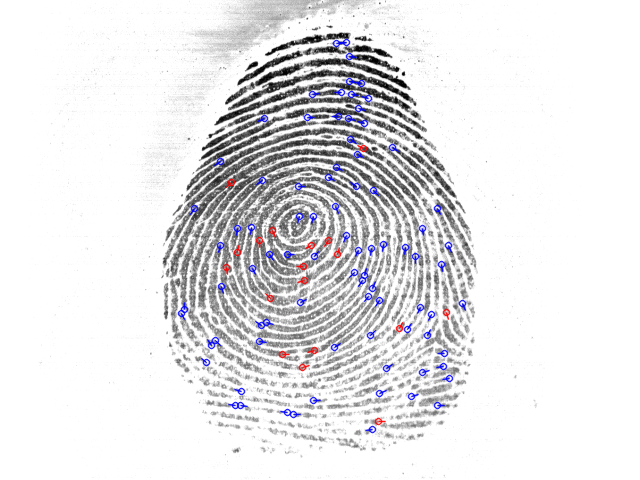
\includegraphics[height=4.0cm]{./image/fingerprint1_1/mnt_overlay.png}\vspace{8pt}
                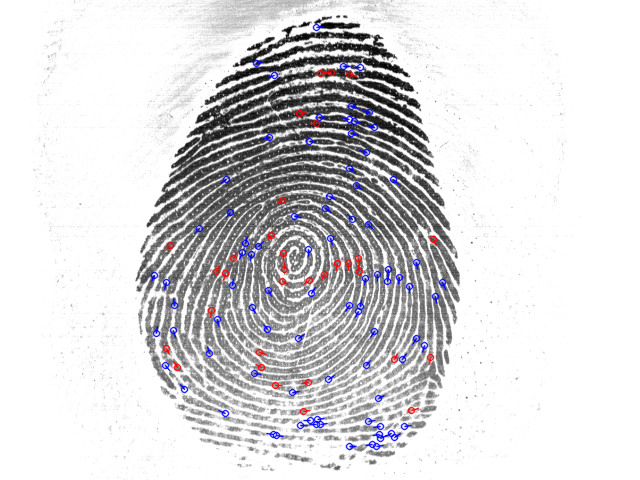
\includegraphics[height=4.0cm]{./image/fingerprint1_2/mnt_overlay.png}\vspace{8pt}
                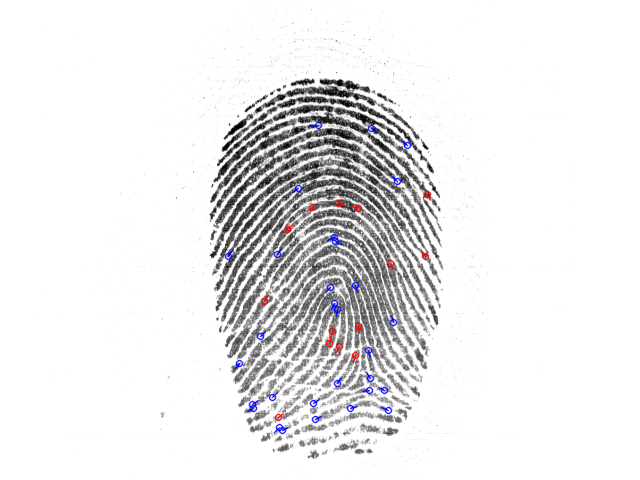
\includegraphics[height=4.0cm]{./image/fingerprint2_1/mnt_overlay.png}
            \end{minipage}
        }
        \hfill
        \subfloat[minutiae connected by triangulation]{
            \begin{minipage}[b]{0.27\linewidth}
                \centering
                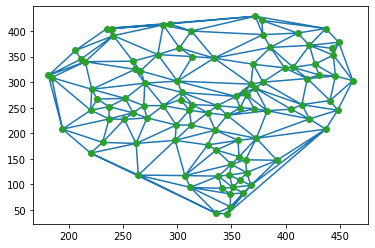
\includegraphics[width=\linewidth, height=4.0cm]{./image/fingerprint1_1/triangulation.png}\vspace{8pt}
                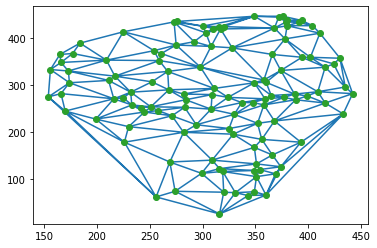
\includegraphics[width=\linewidth, height=4.0cm]{./image/fingerprint1_2/triangulation.png}\vspace{8pt}
                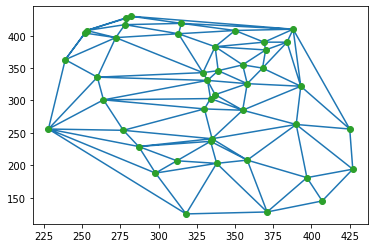
\includegraphics[width=\linewidth, height=4.0cm]{./image/fingerprint2_1/triangulation.png}
            \end{minipage}
        }
        \hfill
        \subfloat[minutiae graph visualization]{
            \begin{minipage}[b]{0.27\linewidth}
                \centering
                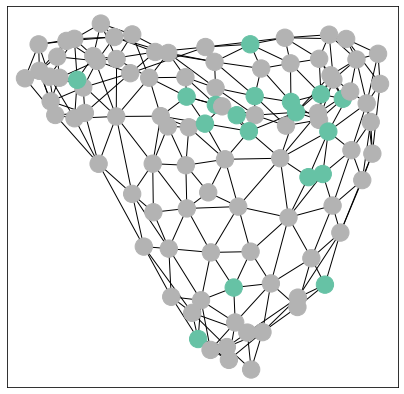
\includegraphics[width=\linewidth, height=4.0cm]{./image/fingerprint1_1/mnt_graph.png}\vspace{8pt}
                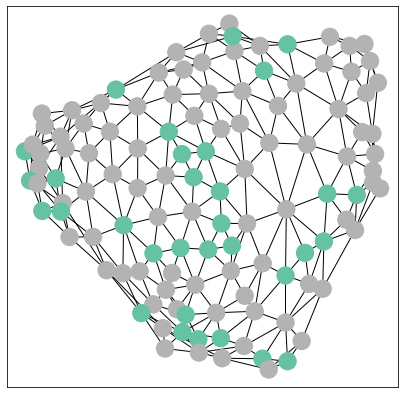
\includegraphics[width=\linewidth, height=4.0cm]{./image/fingerprint1_2/mnt_graph.png}\vspace{8pt}
                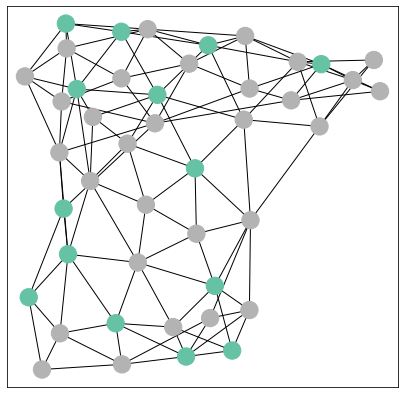
\includegraphics[width=\linewidth, height=4.0cm]{./image/fingerprint2_1/mnt_graph.png}
            \end{minipage}
        }
    \end{minipage}
    \vfill
    \caption{Sample fingerprint and its corresponding minutiae graph}
    \label{fig:mnt}
\end{figure*}

Figure \ref{fig:mnt} illustrates the way we build the minutiae graph. Each row shows one sample fingerprint image with detected minutiae and its corresponding minutiae graph. The left column shows the original fingerprint with detected minutiae that are plotted on it. The middle column shows the minutiae that are connected by Delaunay triangulation method. Note that because the origin of the fingerprint image is on the top left and the origin of the plot is on the bottom left, the minutiae that are plotted in the middle column are turned upside down compared with those minutiae in the left column. The right column shows the minutiae graph once the vertices and edges are built from the previous two columns. The geometric information of the minutiae is lost in the minutiae graph.
    \section{Experiments and Results}
\label{sec:experiment}

\subsection{Training Data Preparation}

We first tried to use NBIS \cite{NBIS} to mark the ground truth minutiae and use it for training.
However, we found that the minutiae detection accuracy of NBIS is low.
It will output an image quality number together with the minutiae location and we can set a threshold to select minutiae.
However, the accuracy is low and if we set a high threshold, then many correct minutiae could not be detected, such as the image shown in Fig. \ref{subfig:NBIS-high}.
And if we set a higher threshold, then it will detect many wrong minutiae, as shown in Fig. \ref{subfig:NBIS-low}.
Besides, it cannot find an accurate minutiae threshold, as it either detected a lot of wrong minutiae or miss many important minutiae, or both.
In addition, the locations of much minutiae were wrongly labeled.
For example, in Fig. \ref{subfig:NBIS-low}, three minutiae locations was not correct and we highlight them using yellow color, and we also mark the correct position with red circle.
We can find that there are about 10 pixels gap between the correct minutiae location and those wrongly detected minutiae location, which will make it harder to train a good model.

Therefore, we decide to mark the ground truth minutiae ourselves using labelme \cite{labelme}.
Because it is difficult to find some latent minutiae in the original image, we first enhance the original fingerprint image by estimating the orientation first and then binarizing with the orientations \cite{caoFingerprintImageEnhancement2017}.
After that, we merge the binarized enhanced images with the original images, and then use labelme to manually mark the minutiae on the merged images.
We did not directly use the binarization enhanced images because that there are much wrong minutiae in the enhanced images, therefore we should refer the original images too.
Fig. \ref{subfig:manually-label} presents an example of the the merged images and our manually marked minutiae.
It is the same image as Fig. \ref{subfig:NBIS-low} and \ref{subfig:NBIS-high}, where our manually marked minutiae is much more accurate than them.

\begin{figure}[htbp]
    \centering
    \subcaptionbox{Minutiae detected by NBIS (with a high quality threshold)\label{subfig:NBIS-high}}{
        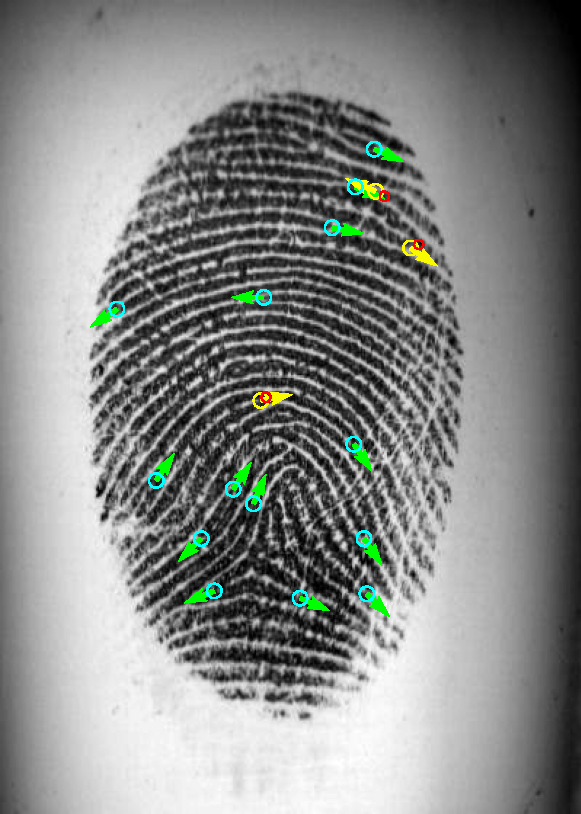
\includegraphics[width=.3\linewidth]{fig/label/nbis-high-thre.pdf}
    }
    \quad
    \subcaptionbox{Our manually marked minutiae\label{subfig:manually-label}}{
        \includegraphics[width=.3\linewidth]{fig/label/manually.png}
    }
    \quad
    \subcaptionbox{Minutiae detected by NBIS (with a low quality threshold)\label{subfig:NBIS-low}}{
        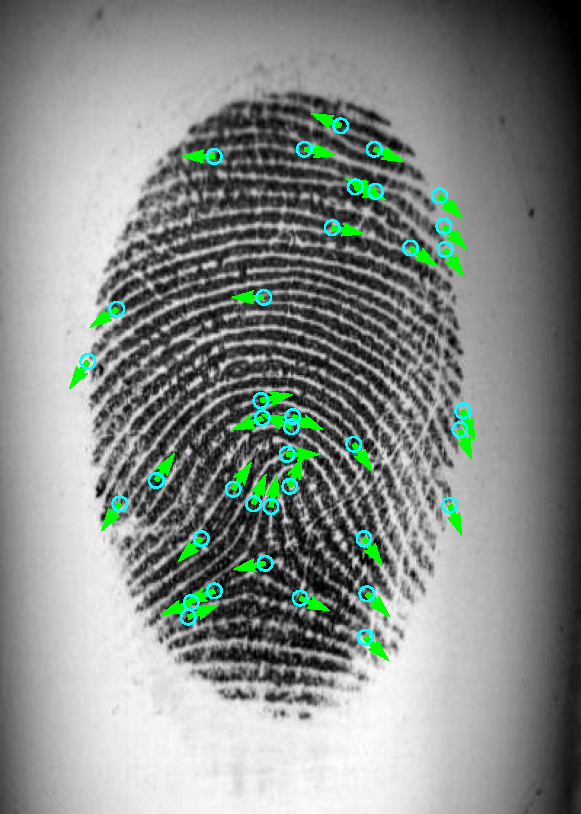
\includegraphics[width=.3\linewidth]{fig/label/nbis-low-thre.pdf}
    }
    \caption{A sample manually marked minutiae with corresponding NBIS detected minutiae}
    \label{fig:label}
\end{figure}


As a result, we first manually selected 200 fingerprint images from the FVC2006 dataset \cite{FVC2006} and marked them manually.
Because we thought these images were not enough and therefore we also manually selected 300 more different high quality fingerprint images which minutiae detection are relatively accurate.
These images are all very clear and the most minutiae was detected by minutiae.
We set a high threshold (35) to filter the incorrect minutiae and get the ground truth minutiae (although there was some missed minutiae and little wrongly detected minutiae).

\def\subwidth{.3}
\begin{figure}[htbp]
    \centering
    \begin{minipage}{.48\linewidth}
        \subcaptionbox{
            original image
        }{
            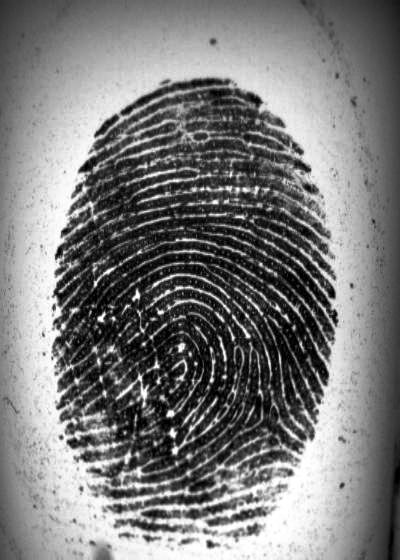
\includegraphics[width=\subwidth\linewidth]{fig/mask/ori-0.png}
        }
        \subcaptionbox{
            minutiae map
            \label{subfig:not-good-1}
        }{
            
\includegraphics[width=\subwidth\linewidth]{fig/mask/mask-0.png}
        }
        \subcaptionbox{
            merged image
        }{
            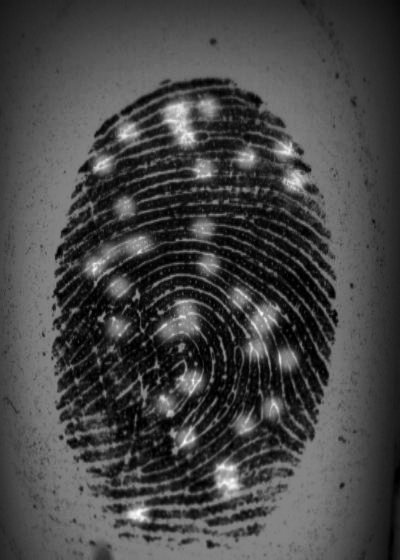
\includegraphics[width=\subwidth\linewidth]{fig/mask/merge-0.png}
        }
    \end{minipage}
    \quad
    \begin{minipage}{0.48\linewidth}
        \subcaptionbox{
            original image
        }{
            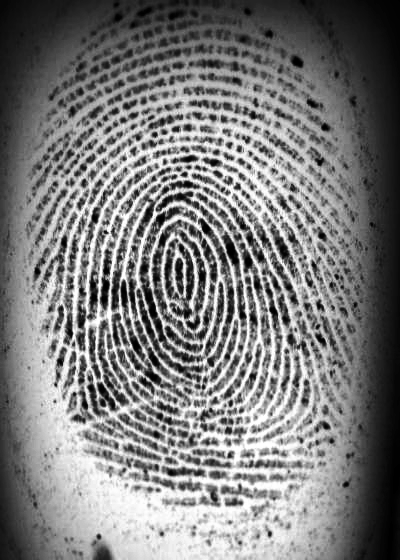
\includegraphics[width=\subwidth\linewidth]{fig/mask/ori-1.png}
        }
        \subcaptionbox{
            minutiae map
        }{
            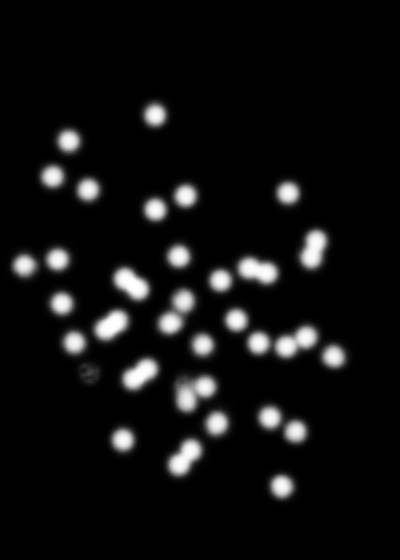
\includegraphics[width=\subwidth\linewidth]{fig/mask/mask-1.png}
        }
        \subcaptionbox{
            merged image
            \label{subfig:good-1}
        }{
            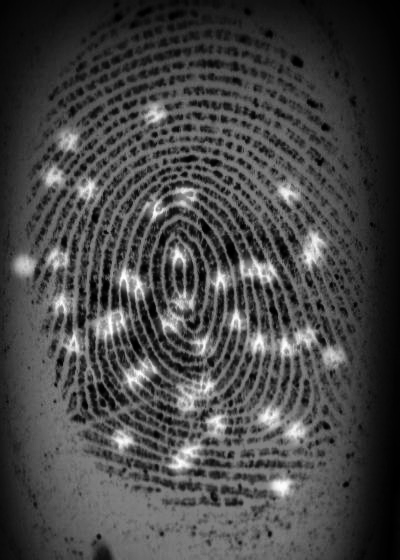
\includegraphics[width=\subwidth\linewidth]{fig/mask/merge-1.png}
        }
    \end{minipage}
    \newline
    \begin{minipage}{.48\linewidth}
        \subcaptionbox{
            original image
        }{
            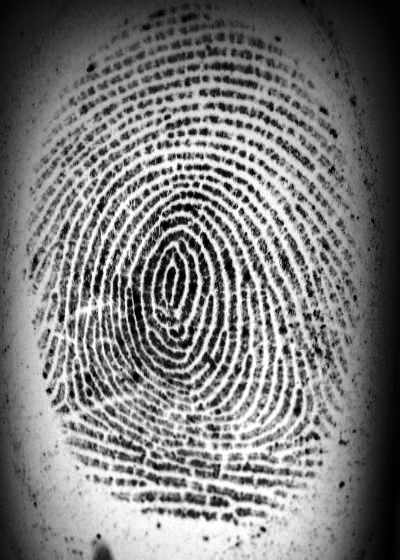
\includegraphics[width=\subwidth\linewidth]{fig/mask/ori-2.png}
        }
        \subcaptionbox{
            minutiae map
            }{
            
\includegraphics[width=\subwidth\linewidth]{fig/mask/mask-2.png}
        }
        \subcaptionbox{
            merged image
            \label{subfig:good-2}
        }{
            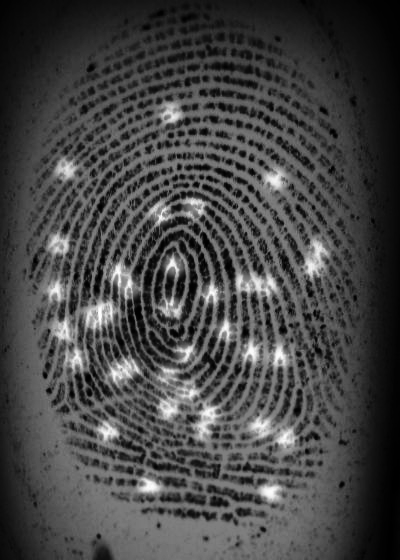
\includegraphics[width=\subwidth\linewidth]{fig/mask/merge-2.png}
        }
    \end{minipage}
    \quad
    \begin{minipage}{0.48\linewidth}
        \subcaptionbox{
            original image
        }{
            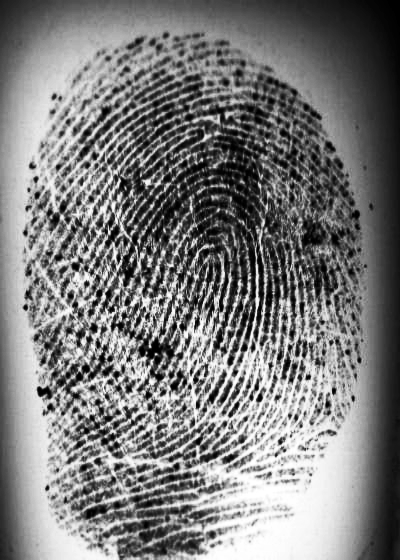
\includegraphics[width=\subwidth\linewidth]{fig/mask/ori-3.png}
        }
        \subcaptionbox{
            minutiae map
        }{
            
\includegraphics[width=\subwidth\linewidth]{fig/mask/mask-3.png}
        }
        \subcaptionbox{
            merged image
            \label{subfig:not-good-2}
        }{
            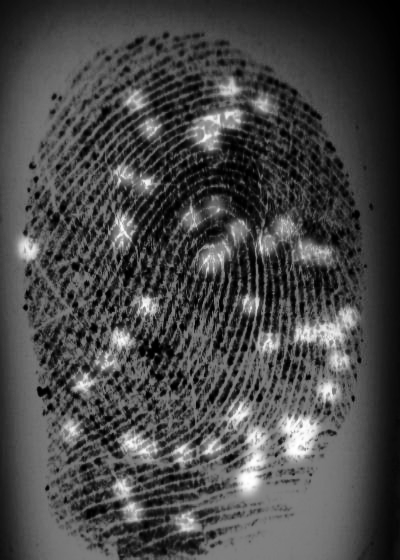
\includegraphics[width=\subwidth\linewidth]{fig/mask/merge-3.png}
        }
    \end{minipage}

    \caption{Some sample images and predicted minutiae map}
    \label{fig:minutiae-map}
\end{figure}


\subsection{Minutiae Detection}

We test our model using the rest of the fingerprint images in FVC2006 dataset.
Fig \ref{fig:minutiae-map} presents some randomly selected sample images and corresponding minutiae map.
We also merge the original images and the predicted minutiae map to make it more clear to view.
From Fig. \ref{fig:minutiae-map}, we can find that the minutiae in sub-figure \ref{subfig:good-1} and \ref{subfig:good-2} are very accurate.
Almost every minutiae is detected and there is not wrongly detected minutiae.
The minutiae in \ref{subfig:not-good-1} and \ref{subfig:not-good-2} is a little worse, where a few minutiae in the noisy area is wrongly detected.

The minutiae detection results are much better than existing algorithms, such as MinutiaeNet \cite{NguyenICB2018}.
We used the source code provided in \cite{NguyenICB2018} and calculate the corresponding minutiae.
Fig. \ref{fig:minutiaenet-results} presents some sample minutiae detection results.
We can easily find that there is a lot of wrongly detected minutiae and missed minutiae.
Due to the time limitation, we did not implement other deep learning based algorithms and make comparison, but based on the detection results, we think our minutiae detection network achieve a very high accuracy and may surpass many existing minutiae detection algorithms.
% , therefore we refer the minutiae detection results in the papers and make a simple comparison.

\def \figwidth {.19}
\begin{figure}[htbp]
    \centering
    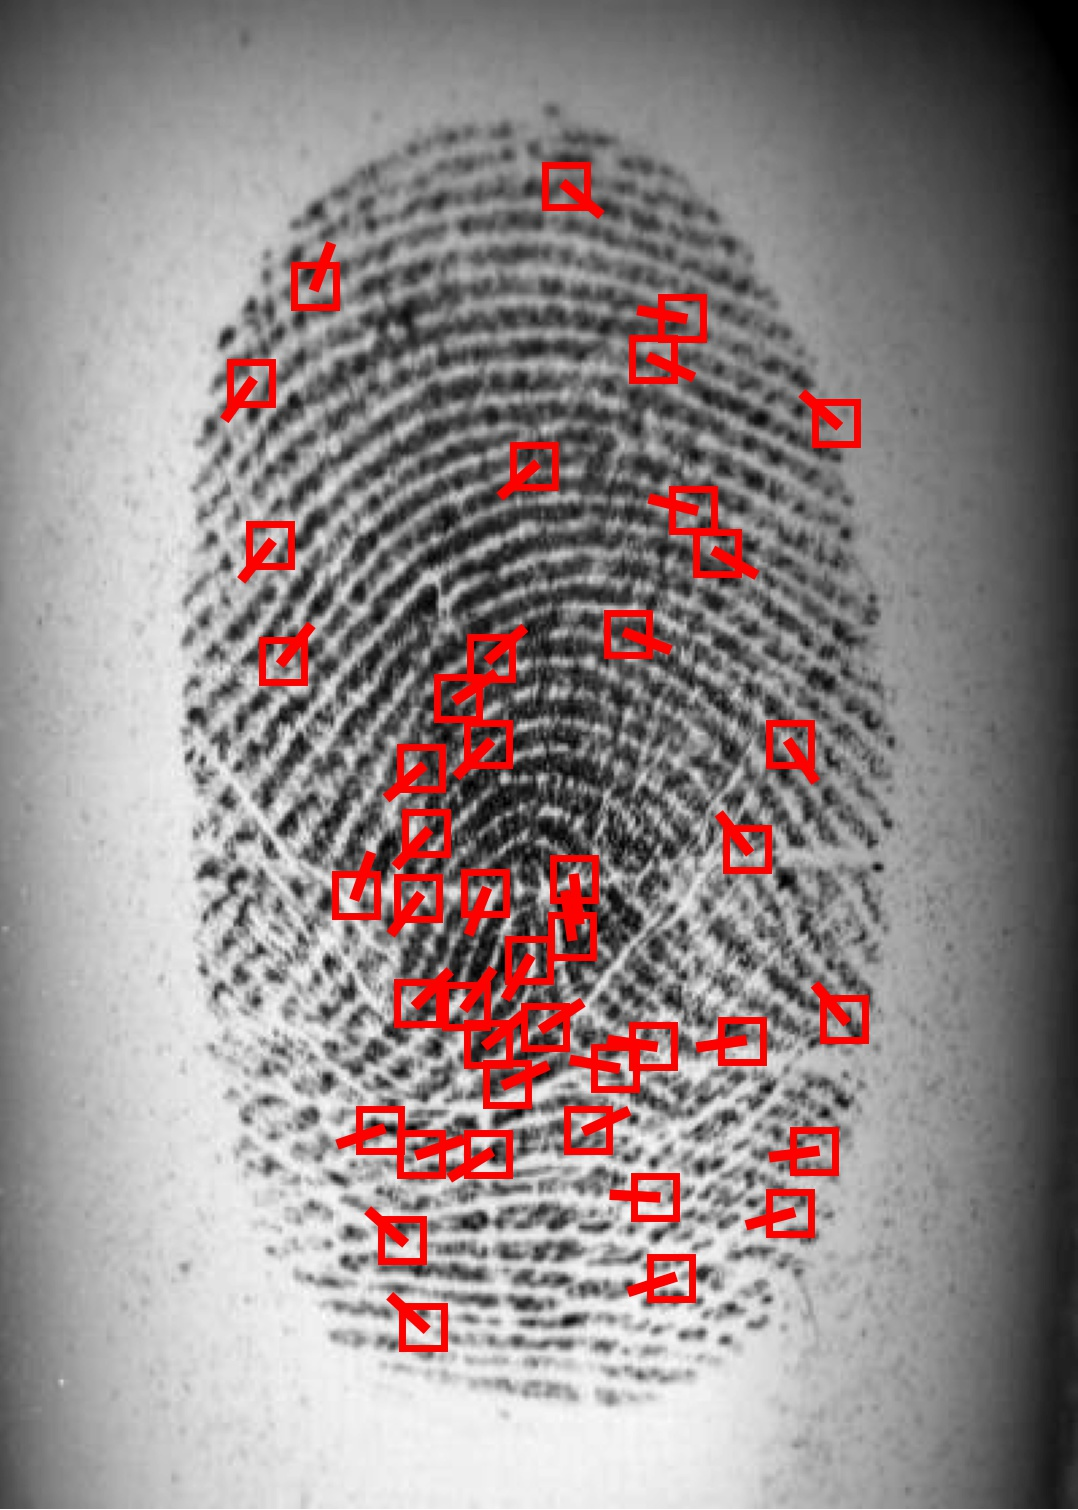
\includegraphics[width=\figwidth\linewidth]{fig/minutiaenet/1.jpg}
    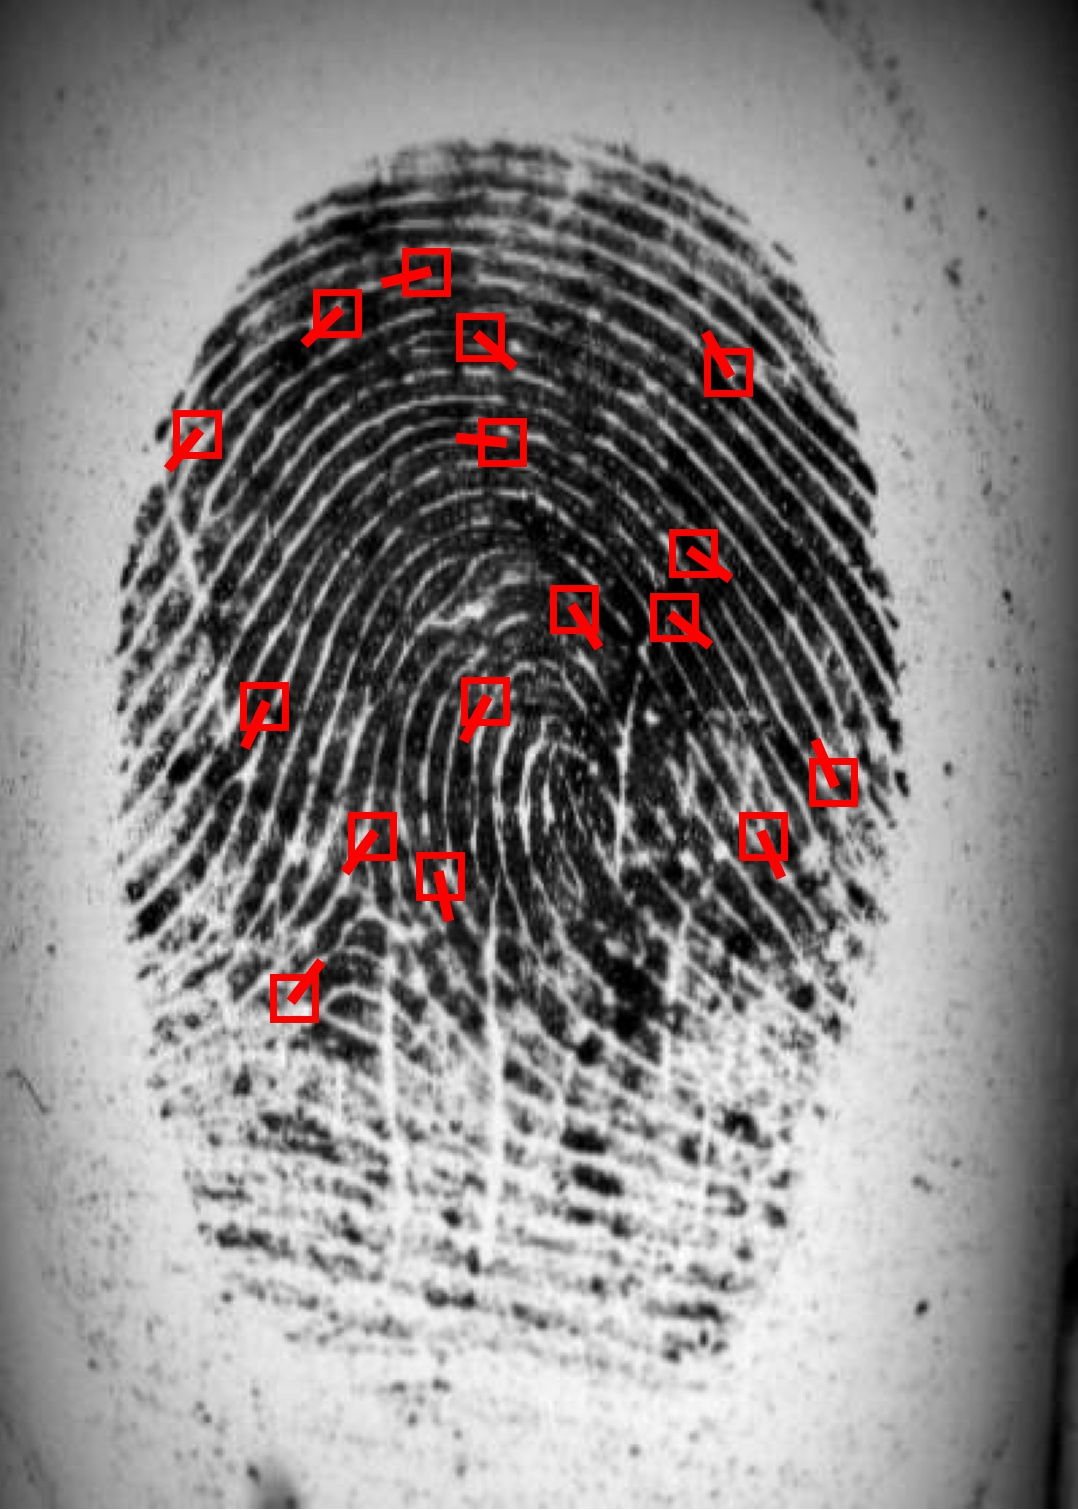
\includegraphics[width=\figwidth\linewidth]{fig/minutiaenet/2.jpg}
    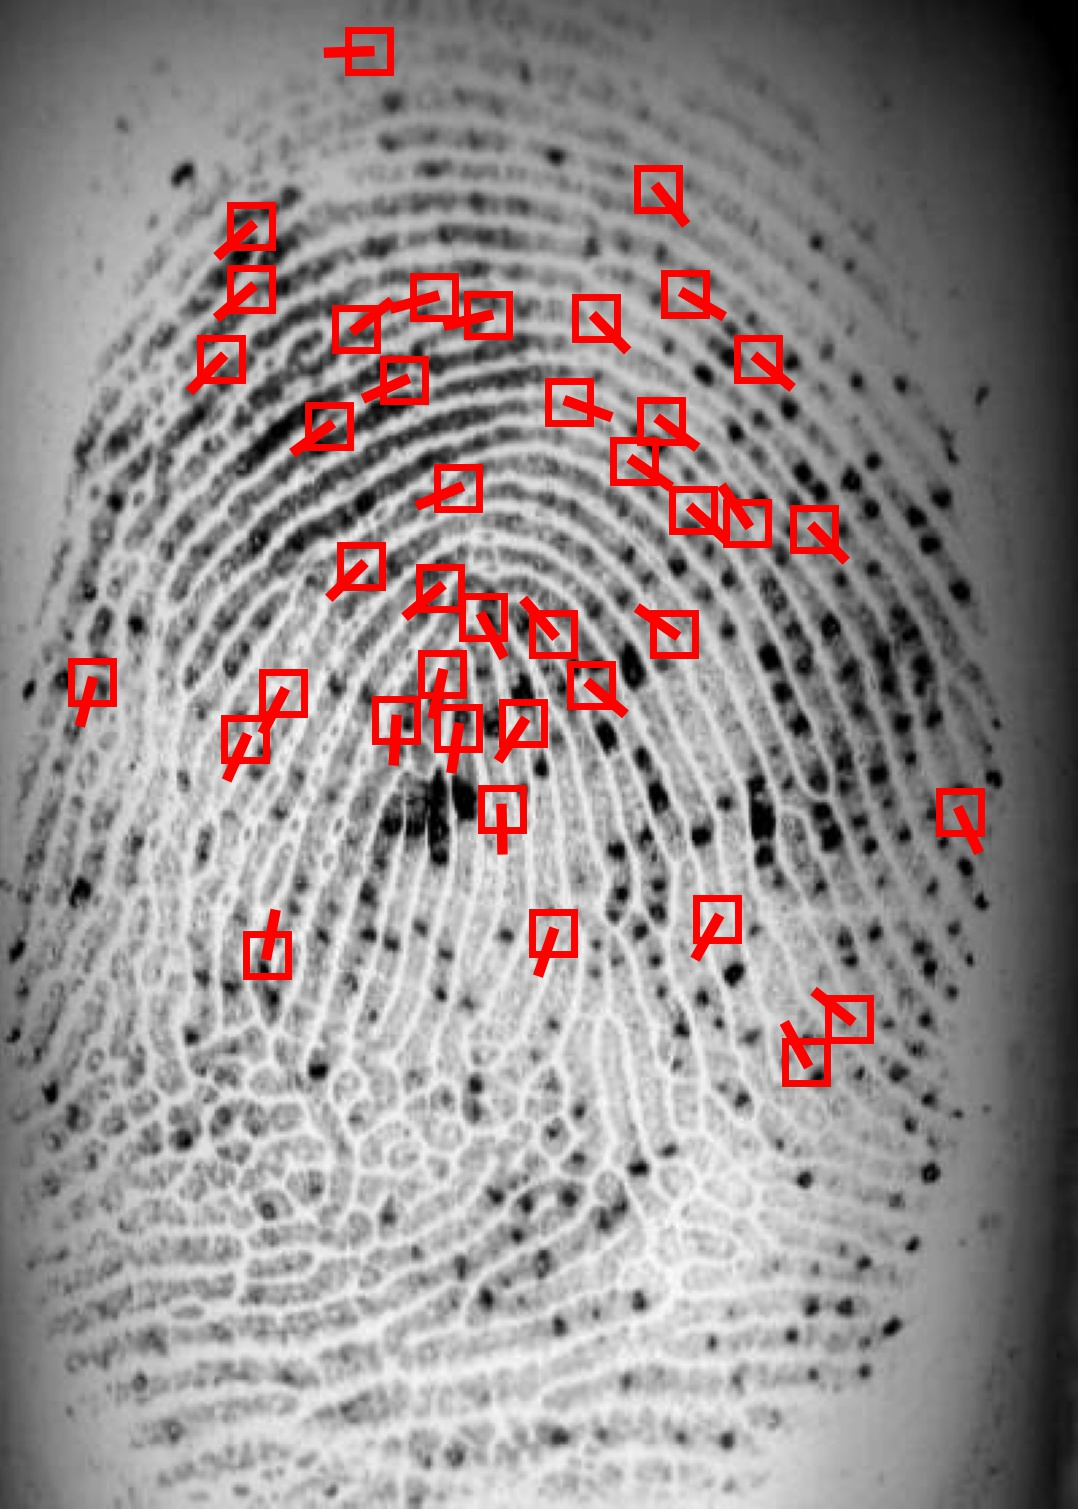
\includegraphics[width=\figwidth\linewidth]{fig/minutiaenet/3.jpg}
    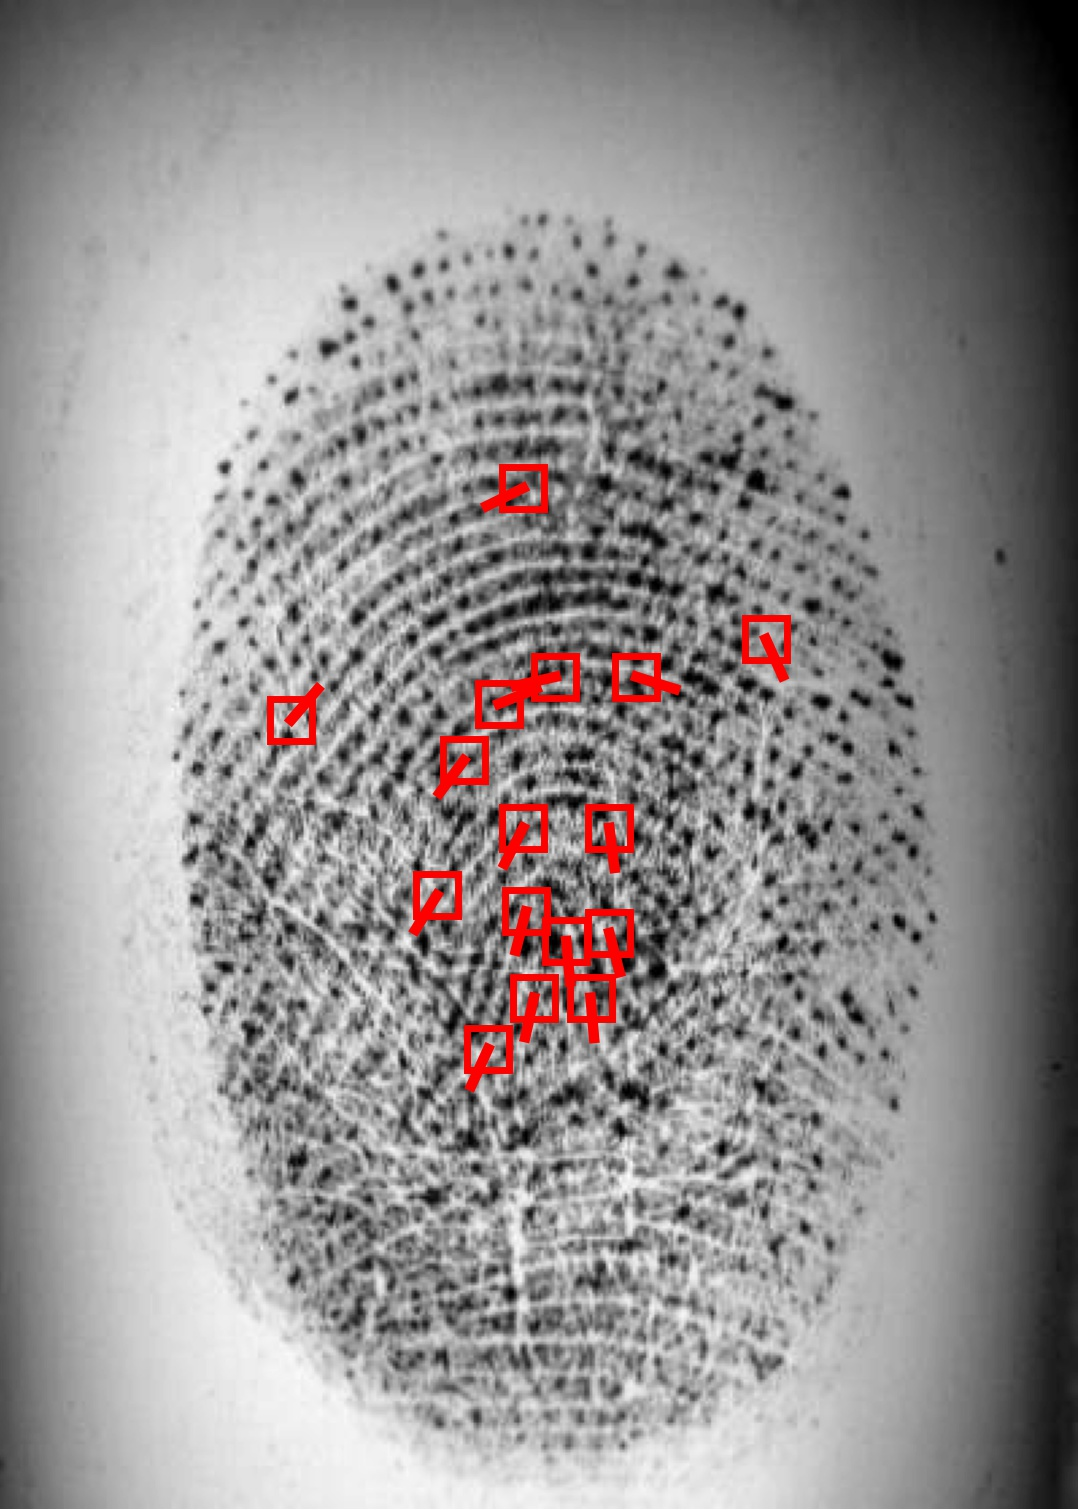
\includegraphics[width=\figwidth\linewidth]{fig/minutiaenet/4.jpg}
    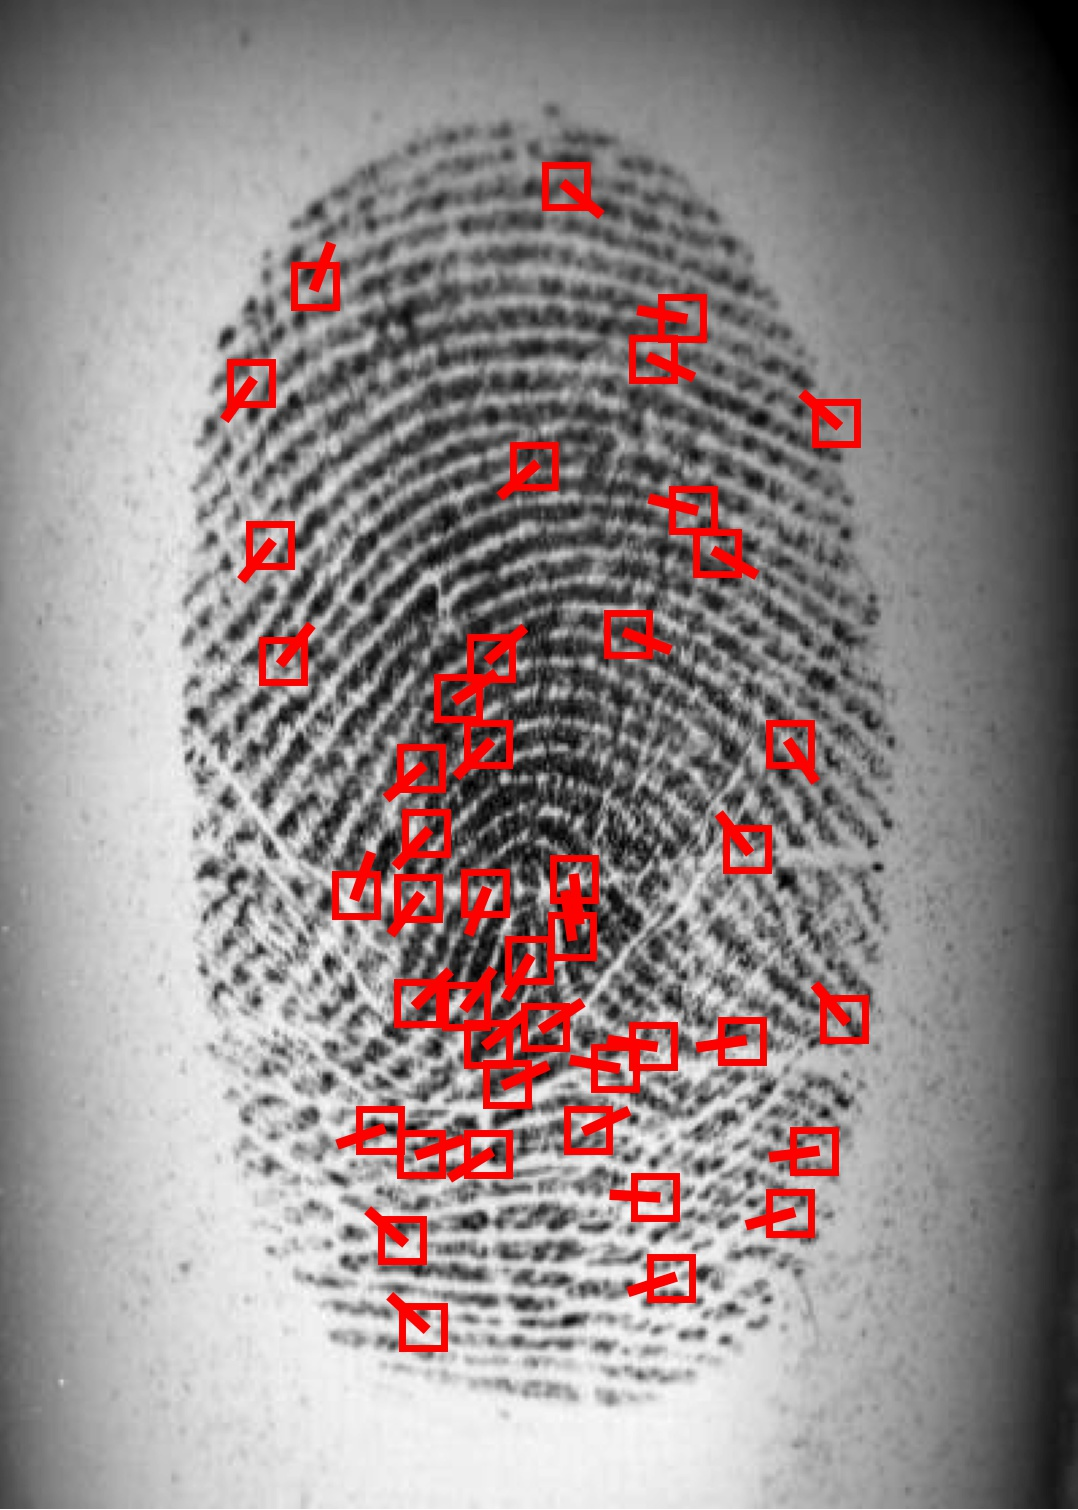
\includegraphics[width=\figwidth\linewidth]{fig/minutiaenet/5.jpg}
    \caption{Some sample minutiae detection results of MinutiaeNet \cite{NguyenICB2018}}
    \label{fig:minutiaenet-results}
\end{figure}

% After detect the minutiae, we then use non maximum suppression to locate the minutiae.




\subsection{Graph Triplet}

We use MNIST dataset \cite{LecunIEEE1998} to build the graph triplet, and use SplineCNN layer \cite{FeyCVPR2018splinecnn} \cite{FeyICLR2020DGMC} to replace the CNN layer which is normally used in computer vision task. Each MNIST image is represented as a graph, whose nodes correspond to the pixels in the image and the edge is formed by connected each pixel to all its neighboring pixels. Therefore, based on this setup, each MNIST image is a graph with the same number of nodes, which is $784(=28^2)$. The graph triplet is formulated as follows: for each sample as the anchor in the training dataset, we randomly select another sample which belongs to the same class as the positive sample, and randomly select one sample from the rest classes as the negative sample. 

Similar to CNN neural network configuration, we build a SplineCNN network, which contains two SplineCNN layers, and ech SplineCNN layer is followed by an exponential linear unit (ELU) and a max-pooling layer. There are two fully connected layers, the first fully connected layer is also followed by an ELU layer, the output dimension of the final fully connected layer is $10$ (we also choose the final dimension to be $2$ for visualization). The initial learning rate is $10^{-3}$. Stochastic gradient descent with Adam method is used for optimization and the total training epochs is $20$.

\begin{figure}[htb]
    \begin{minipage}[b]{0.48\linewidth}
        \centering
        \centerline{\epsfig{figure=./image/mnist_plot/train_plot.png, height=7.0cm}}
        % \caption{MNIST training set result}
        % \label{fig:mnist_train_plot}
    \end{minipage}
    \hfill
    \begin{minipage}[b]{0.48\linewidth}
        \centering
        \centerline{\epsfig{figure=./image/mnist_plot/test_plot.png, height=7.0cm}}
        % \caption{MNIST test set result}
        % \label{fig:mnist_test_plot}
    \end{minipage}
    \caption{Visualization of MNIST training set and test set result}
    \label{fig:mnist_plot}
\end{figure}

For evaluation, since the total number of samples of MNIST test dataset is $10,000$ and they are not balanced for each class, we randomly choose 500 samples from each class. We use all-to-all evaluation protocol, which means for each test sample, Euclidean distance is computed against all the rest samples. Therefore, in total, we generate $1,247,500$ genuine scores and $11,250,000$ impostor scores. Since MNIST dataset is a simple dataset with a few number of classes and a large number of samples for each class, it turns out that there is no overlap between genuine scores and impostor scores. The equal error rate(EER) is thus zero.


    \section{Conclusion and Future Work}
\label{sec:conclusion}

In this paper, we have


There are several directions that deserve to explore in the future: 
    

\bibliographystyle{plain}
\bibliography{ref}

\end{spacing}
\end{document}

 